\documentclass[a4paper,12pt]{article} % Copyright (c) 2020  Brian Schubert
\usepackage{amsmath,amsthm,amsfonts,amssymb}
\usepackage{titling}
\usepackage{enumitem}
\usepackage{geometry}
\usepackage[makeroom]{cancel}
\usepackage{tikz}
\usepackage{pgfplots}

% For problem 3b
\usepgfplotslibrary{groupplots}

\geometry{left=0.75in,right=0.75in,top=1in,bottom=1in}

\theoremstyle{plain}
\newtheorem{problem}{Problem}

% Hide QED symbol
%\renewcommand{\qedsymbol}{}

\begin{document}
% Title
\begin{center}
    \huge
    Math 4545 Take Home \#1

    \vspace{0.5cm}
    \large
    Brian Schubert

    \vspace{0.5cm}
    Due: 02/21/2020
\end{center}

\begin{problem}
    In class used the F.S.S of $f(x)=1$, $0 \leq x \leq \pi$,
    to show that \begin{equation*}
     1-\frac{1}{3}+\frac{1}{5}-\frac{1}{7}+\cdots = \frac{\pi}{4}.
     \end{equation*} 
     Use the F.C.S of $f(x)=x^2$, $0\leq x \leq \pi$, to find \begin{equation*}
        1 + \frac{1}{2^2} + \frac{1}{3^2} + \frac{1}{4^2} + \cdots
     \end{equation*}
\end{problem}

\begin{proof}[\textbf{Solution}]
    The F.C.S of $f$ is \begin{equation*}
        f(x) \sim \frac{a_0}2 + \sum_{n=1}^\infty a_n \cos \left(nx\right),
        \quad 
        a_0 = \frac{2}{\pi} \int_0^\pi f(x) \, \mathrm dx, \quad
        a_n = \frac{2}{\pi} \int_0^\pi f(x) \cos \left(nx\right) \, \mathrm dx
    \end{equation*}
    Computing the coefficients,
    \begin{align*}
        a_0 &= \frac{2}{\pi} \int_0^\pi x^2 \, \mathrm dx = \frac{2}{\pi} \left[ \frac{1}{3}x^3\right]_0^\pi = \frac{2}{3}\pi^2,\\
        a_n &= \frac{2}{\pi} \int_0^\pi x^2 \cos \left(nx\right) \, \mathrm dx
            = \frac{2}{\pi} \left[ \cancelto{0}{\left.\frac{x^2}{n}\sin(nx)\right|_0^\pi } - \frac{2}{n} \int_0^\pi x \sin (nx)\,\mathrm dx \right] \\
            &=\frac{-4}{\pi n} \left[ \left.\frac{-x}{n}\cos(n x) \right|_0^\pi+ \frac{1}{n} \int_0^\pi  \cos (nx)\,\mathrm dx \right]
            = \frac{-4}{\pi n} \left[ \left(\frac{\pi}{n}(-1)^{n+1}\right) + \cancelto{0}{\left.\left(\frac{1}{n^2}\sin(nx) \right)\right|_0^\pi} \right]\\
            &=\frac{4}{n^2}(-1)^{n}
    \end{align*}
    Therefore, 
    \begin{equation*}
        f(x) = x^2 \sim  \frac{\pi^2}{3} + 4\sum_{n=1}^\infty \left(\frac{1}{n^2 }(-1)^n\right)\cos(nx)
    \end{equation*}
    
    Since this series converges to the even piecewise extension of $f$, the series evaluated at the endpoint $x=\pi$ will equal $f(\pi)$. As such, we can compute:
    \begin{align*}
    &&f(\pi) = \pi^2 &= \frac{\pi^2}{3} + 4\sum_{n=1}^\infty \left(\frac{1}{n^2 }(-1)^n\right)\cos(n\pi) = \frac{\pi^2}{3} + 4\sum_{n=1}^\infty \frac{1}{n^2 }(-1)^n(-1)^n = \frac{\pi^2}{3} + 4\sum_{n=1}^\infty \frac{1}{n^2 } \\
    &\iff& \frac{2\pi^2}{3} & = \hphantom{\frac{\pi^2}{3} +\ } 4\sum_{n=1}^\infty \frac{1}{n^2 } = 4\left(1 + \frac{1}{2^2} + \frac{1}{3^2} + \frac{1}{4^2} + \cdots\right) \\
    &\iff& \frac{1}{4} \cdot \frac{2\pi^2}{3} &= \hphantom{\frac{\pi^2}{3} + 4} \sum_{n=1}^\infty \frac{1}{n^2 } = 1 + \frac{1}{2^2} + \frac{1}{3^2} + \frac{1}{4^2} + \cdots\\
    &\iff& \boxed{\frac{\pi^2}{6}} &= \hphantom{\frac{\pi^2}{3} + 4} \sum_{n=1}^\infty \frac{1}{n^2 } = 1 + \frac{1}{2^2} + \frac{1}{3^2} + \frac{1}{4^2} + \cdots
%    &&f(0) = 0&= \frac{\pi}{2} + \sum_{n=1}^\infty \left(\frac{2}{n^2 \pi}\Big[(-1)^n - 1\Big]\right) \cdot 1 \\
%     &\iff& -\frac{\pi}{2}&=\sum_{n=1}^\infty \left(\frac{2}{n^2 \pi}\Big[(-1)^{n}-1\Big]\right) = \frac{-4}{\pi} + \frac{-4}{3^2\pi} + \frac{-4}{5^2 \pi} + \cdots\\
%    &\iff& \frac{\pi}{2}&=\sum_{n=1}^\infty \left(\frac{2}{n^2 \pi}\Big[1-(-1)^{n+1}\Big]\right) = \frac{4}{\pi} + \frac{4}{3^2\pi} + \frac{4}{5^2 \pi} + \cdots\\
%    &\iff& \frac{\pi}{4}\cdot\frac{\pi}{2}&=\sum_{n=1}^\infty \left(\frac{2}{n^2 \pi}\Big[1-(-1)^{n+1}\Big]\right) = \frac{\pi}{4}\left(\frac{4}{\pi} + \frac{4}{3^2\pi} + \frac{4}{5^2 \pi} + \cdots\right)\\ 
%    &\iff& \boxed{\frac{\pi^2}{8}} &= 1 + \frac{1}{3^2} + \frac{1}{5^2} + \frac{1}{7^2}+\cdots
    \end{align*}
    
\end{proof}

\begin{problem} % 2
    Consider the boundary value problem
    \begin{align*}
        &f'' + \lambda f = 0 &  &0 \leq x \leq \pi \\
        &f(0) = 0 && f(\pi) -2f'(0) = 0
    \end{align*}
    
    \begin{enumerate}[label=\alph*.)]
        \item One of the hypotheses of a SL BVP with separated boundary conditions doesn't hold. Which one?
        \item Is $\lambda =0$ an e-value?
        \item Are there any e-values for $\lambda < 0$? If so find them.
        \item Are there any e-values for $\lambda > 0$? If so find them.
    \end{enumerate}
\end{problem}

\begin{proof}[\textbf{Solution}] % 2
\begin{enumerate}[label=\alph*.)]
    \item For a regular SL-BVP with $x\in (a,b)$, the boundary conditions are defined to be of the form
    \begin{align*}
        \kappa_1 f(a) = \kappa_2 f'(a) = 0,    \qquad       \kappa_3 f(b) + \kappa_4 f'(b) = 0
    \end{align*}
    In the given problem, the second boundary condition is given in terms of both the left- and right-hand boundaries. However, in the expected form, the second boundary condition should be given in terms of only the right-hand boundary.
    
    \item If $\lambda = 0$, then $f = \alpha x + \beta$ and $f' = \alpha$.  \begin{align*}
    \intertext{ Since $f(0)=0$,}
        \alpha \cdot 0+\beta = 0 \implies &\beta = 0  &\text{so}  &  &f=\alpha x \text{ and } f' = \alpha
     \intertext{Since $f(\pi) - 2f'(0) = 0$,}
        \alpha \pi -2\alpha = \alpha(\pi-2) = 0 \implies &\alpha = 0 &\text{so} &  &f \equiv 0
    \end{align*}
    Since $f\equiv 0$ cannot be an eigenfunction, \underline{$\lambda = 0$ is not an eigenvalue for the SL-BVP}.
    
    \item  \underline{For $\lambda < 0$}, let $\lambda = -a^2$. Then $f = C_1 \cosh (a x) + C_2 \sinh (ax)$ and \\ \hspace*{2.06in} $f' =  C_1 a\sinh (a x) + C_2 a\cosh (ax)$.
    
    Since $f(0)=0$,
    \begin{align*}
        &&f(0) = C_1 \cosh (0) + C_2 \sinh (0) &= 0\\
        &\iff& C_1 \cdot 1 + C_2 \cdot 0 &= 0 \\
        &\iff& C_1 &= 0 &\text{so} &  &\begin{cases}
        f=C_2 \sinh(ax), \\ f'=C_2a\cosh(ax)\end{cases}
    \intertext{Since $f(\pi) - 2f'(0) = 0$,}
        &&f(\pi) - 2f'(0) = \cancel{C_2} \sinh(a\pi) - 2\cancel{C_2} a\cdot 1 &= 0 \\
        &\iff& \sinh(a\pi) &= 2a
    \end{align*}
    
    Therefore, the eigenvalues $\lambda < 0$ will be the solutions to the transcendental equation $\sinh (a \pi) = 2a$, $a=\sqrt{-\lambda}$. To find these solutions, we consider the graphs of both sides of the equation, $y_1 = \sinh (a\pi)$ and $y_2 = 2a$. Since at  $a=0$ (outside the domain of consideration), $y_1(0) = y_2(0)=0$, the origin is contained in graphs of both. For $a>0$, we note that \begin{equation*}
    y'_1 = \pi \cosh (a \pi) > \pi >  y'_2 = 2. 
    \end{equation*}
    Since $y_1$ always increases faster than $y_2$ on the interval, there will be no intersections for $a>0$. Therefore, \underline{there are no eignenvalues  $\lambda < 0$}. This result is confirmed graphically by plotting $y_1$ and $y_2$:
    
    \begin{center}
        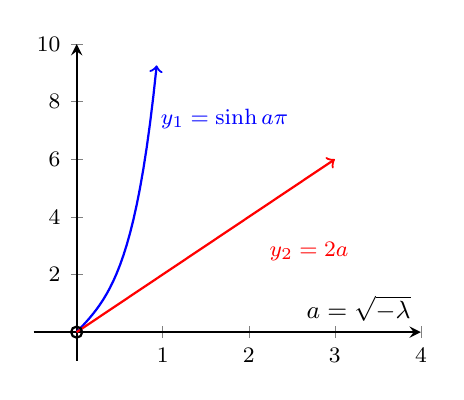
\begin{tikzpicture}
        \begin{axis}[
        axis lines=center,
        xlabel={$a=\sqrt{-\lambda}$},
%        xlabel style={below midway},
        ylabel style={above left},
        xmin=-0.5,
        xmax=4,
        ymin=-1,
        ymax=10,
        thick,
        small,
        ] 
        \addplot+[->, mark=none, domain=0:0.93] {sinh(x*pi)} node[pos=0.8, right]
         {\footnotesize $y_1=\sinh{a\pi}$}; 
         
         
        \addplot+[->, mark=none, domain=0:3] {2*x} node[pos=0.9, below, yshift=-20] {\footnotesize $y_2=2a$};
        \addplot[mark=o] coordinates {(0,0)};
        \end{axis}
        \end{tikzpicture}
    \end{center}
    
    \item \underline{For $\lambda > 0$}, \begin{equation*}
        f=C_1 \cos \left(\sqrt{\lambda}x\right) + C_2 \sin\left(\sqrt{\lambda}x\right), \qquad
        f'=-C_1 \sqrt{\lambda}\sin \left(\sqrt{\lambda}x\right) + C_2 \sqrt{\lambda}\cos\left(\sqrt{\lambda}x\right)
    \end{equation*}
    \begin{align*}
    \intertext{Since $f(0)=0$,}
        C_1 \cdot 1 + C_2 \cdot 0 = 0 \implies &C_1 = 0 &\text{so} &  &\begin{cases}
        f=C_2 \sin(\sqrt{\lambda}x), \\ f'=C_2\sqrt{\lambda}\cos(\sqrt{\lambda}x)\end{cases}
    \intertext{Since $f(\pi) - 2f'(0) = 0$,}
        \cancel{C_2} \sin(\sqrt{\lambda}\pi) - 2\cancel{C_2} \sqrt{\lambda}\cdot 1 = 0 \implies &\sin(\sqrt{\lambda}\pi) = 2\sqrt{\lambda} &&&
    \end{align*}
    Therefore, the eigenvalues $\lambda > 0$ will be the solutions to the transcendental equation $\sin (\sqrt{\lambda} \pi) = 2\sqrt{\lambda}$. These solutions can be found graphically by ploting $y_1=\sin (\sqrt{\lambda} \pi)$ and $y_2 =  2\sqrt{\lambda}$:
    
    \begin{center}
        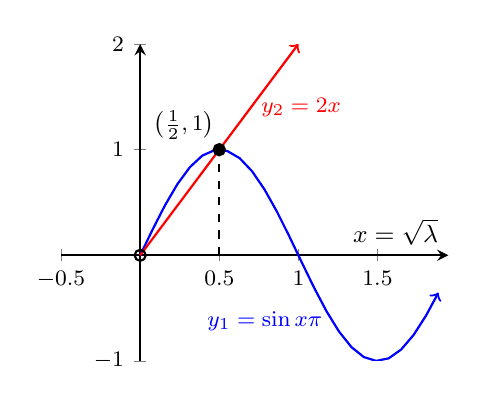
\begin{tikzpicture}
        \begin{axis}[
        axis lines=center,
        xlabel={$x=\sqrt{\lambda}$},
        %        xlabel style={below midway},
        ylabel style={above left},
        xmin=-0.5,
        xmax={0.62*pi},
        ymin=-1,
        ymax=2,
        thick,
        small,
        ] 
        \addplot+[->, mark=none, domain=0:0.6*pi] {sin(deg(x*pi))} node[pos=0.7, left]
        {\footnotesize $y_1=\sin{x\pi}$}; 
        \addplot+[->, mark=none, domain=0:1] {2*x} node[pos=0.7, right] {\footnotesize $y_2=2x$};
        \addplot[mark=o] coordinates {(0,0)};
        \addplot[mark=*] coordinates {(0.5,1)} node[above left, xshift=2] {\footnotesize $\left(\frac{1}{2}, 1\right)$};
        \addplot[mark=none, dashed] coordinates {(0.5, 0)  (0.5, 1)};
        \end{axis}
        \end{tikzpicture}
    \end{center}
    This plot indicates that the only solution is $\sqrt \lambda = \frac{1}{2}$.
    
    Therefore, for $\lambda > 0$, the only eignenvalue is $\lambda_1 = \frac{1}{4}$, with a corresponding eigenfunction of $f_1 \sim \sin \left( \frac{x}{2} \right)$
    
\end{enumerate}
\end{proof}


\begin{problem} % 3
    Consider the boundary value problem
    \begin{align*}
    &f'' + \lambda f = 0 &  &0 \leq x \leq \pi \\
    &f(0) + f'(0) = 0 && f(\pi) -f'(\pi) = 0
    \end{align*}
    
    \begin{enumerate}[label=\alph*.)]
        \item Determine if there are \underline{negative} e-values, and if so display them graphically and estimate.
        \item State what happens to the negative e-value(s) of this SL BVP if the right end point is $p$ where $p>\pi$.
    \end{enumerate}
\end{problem}

\begin{proof}[\textbf{Solution}] % 3
    \begin{enumerate}[label=\alph*.)]
        \item  \underline{For $\lambda < 0$}, let $\lambda = -a^2$, $a>0$. Then \begin{equation*}
        f = C_1 \cosh (a x) + C_2 \sinh (ax), \qquad f' =  C_1 a\sinh (a x) + C_2 a\cosh (ax).
        \end{equation*}
        
        Since $f(0) + f'(0) = 0$,
        \begin{align*}
            &&&f(0) + f'(0) = C_1 \cosh 0 + C_2 \sinh 0 + C_1 a \sinh 0 + C_2 a \cosh 0 = 0\\
            &\iff& &C_1 + C_2 a = 0 \\
            &\iff& &C_1 = -C_2 a  \qquad \text{so}\qquad \begin{cases}
                f=-C_2 a \cosh (ax) + C_2 \sinh(ax),\\
                f'=-C_2 a^2 \sinh(ax) + C_2 a \cosh(ax)
            \end{cases}
        \end{align*}
        Since $f(\pi) -f'(\pi) = 0$, and $C_2 \neq 0$,
        \begin{align*}
            && &f(\pi) - f'(\pi) = \Big(-C_2a \cosh (a\pi) + C_2 \sinh (a\pi)\Big) - \Big(-  C_2a^2\sinh (a \pi) + C_2 a\cosh (a\pi)\Big) =0 \\
            &\iff&& -a \cosh(a\pi) + \sinh(a\pi) + a^2 \sinh(a\pi) - a \cosh(a\pi) = 0\\
            &\iff&& (-2a)\cosh(a\pi) + (1+a^2)\sinh(a\pi) = 0\\
            \intertext{Since $\cosh(a\pi) \neq 0$,},
            &&&(-2a)\frac{\cosh(a\pi)}{\cosh(a\pi)} + (1+a^2)\frac{\sinh(a\pi)}{\cosh(a\pi)} = 0 \\
            &\iff& &-2a+(1+a^2)\tanh(a\pi) = 0 \\
            &\iff&& \tanh (a\pi) = \frac{2a}{1+a^2}
        \end{align*}
        
        Therefore, the eignevalues $\lambda <0$ are the solutions to the transcendental equation $\tanh (a\pi) = 2a/(1+a^2)$, $a=\sqrt{-\lambda}$. These solutions may be found graphically by plotting $y_1 = \tanh (a\pi) - 2a/(1+a^2)$ and determining the intercepts with the $x$-axis:
        \begin{center}
            \begin{tikzpicture}
            \begin{axis}[
            axis lines=center,
            xlabel={$a=\sqrt{-\lambda}$},
            xlabel style={right},
            ylabel style={above left},
            xmin=-2.0,
            xmax=2.0,
            ymin=-0.3,
            ymax=0.3,
            thick,
            samples=100,
            clip=false,            
            ]
            \addplot+[<-, dashed, mark=none, domain=-1.5:0, blue] {(1+\x^2)*tanh(\x*pi) - 2*\x};

            \addplot+[->, mark=none, domain=0:1.5, blue] {tanh(\x*pi) - (2*\x)/(1+\x^2)} node[above right] {\footnotesize $y_1=\tanh(a\pi)-2a/(1+a^2)$};
            
            \addplot[mark=o] coordinates {(0,0)};
            \addplot[mark=*] coordinates {(0.88225181948493,0) (1.0715068662678,0)};
            \end{axis} 
            \end{tikzpicture}
        \end{center}
        This yields two solutions, $\sqrt{-\lambda_1}\approx 0.88225$ and $\sqrt{-\lambda_2}\approx 1.07151$.
    
    \item As the right end points $p$ increases, the two intercepts found above grow closer to $\sqrt{-\lambda}=a=1$:
    
    \begin{center}
        \begin{tikzpicture}
        \begin{groupplot}[group style={
                group name=myplot,
                vertical sep=2cm,
                horizontal sep=2cm,
                group size= 2 by 2,
            },
            ymax=0.5,
            height=5cm,
            width=6.4cm
            ]
            
        \nextgroupplot[title={$p=\pi$}, axis lines=center, samples=100,
            legend to name=firstplot
        ]
         % (Relative) Coordinate at top of the first plot
        \coordinate (c1) at (rel axis cs:0,1);
        \addplot+[->, mark=none, domain=0:1.5, blue] {tanh(\x*pi) - (2*\x)/(1+\x^2)};
        \addplot[mark=o] coordinates {(0,0)};
        \addplot[mark=*] coordinates {(0.88225181948493,0) (1.0715068662678,0)};
        \addlegendentry{$\tanh(ap)-\frac{2a}{1+a^2}$}
        
        \nextgroupplot[title={$p=1.2\pi$}, axis lines=center, samples=100]
        % (Relative) Coordinate at top of the second plot
        \coordinate (c2) at (rel axis cs:1,1);
        \addplot+[->, mark=none, domain=0:1.5, blue] {(1+\x^2)*tanh(\x*1.2*pi) - 2*\x};
        \addplot[mark=o] coordinates {(0,0)};
        \addplot[mark=*] coordinates {(0.9447906,0) (1.040395,0)};
        
        \nextgroupplot[title={$p=1.5\pi$}, axis lines=center, samples=100]
        \addplot+[->, mark=none, domain=0:1.5, blue] {tanh(\x*1.5*pi) - (2*\x)/(1+\x^2)};
        \addplot[mark=o] coordinates {(0,0)};
        \addplot[mark=*] coordinates {(0.9804959,0) (1.01674,0)};
        
        \nextgroupplot[title={$p=2\pi$}, axis lines=center, samples=100]
        \addplot+[->, mark=none, domain=0:1.5, blue] {tanh(\x*2*pi) - (2*\x)/(1+\x^2)};
        \addplot[mark=o] coordinates {(0,0)};
        \addplot[mark=*] coordinates {(0.996182,0) (1.0036567,0)};
        
        \end{groupplot}
        % Sigle legened solution from
        % https://tex.stackexchange.com/questions/315224/center-legend-above-or-below-a-groupplot-without-references
        \coordinate (c3) at ($(c1)!.5!(c2)$);
        \node[below] at (c3 |- current bounding box.south)
        {\pgfplotslegendfromname{firstplot}};
        \end{tikzpicture}
    \end{center}
    
    Therefore, for right end points $p$ large, the eignenvalues $\lambda <0$ approach $-1$.
    \end{enumerate}
\end{proof}

\end{document}

